\documentclass[margin=1cm]{standalone}
\usepackage{tikz}
\usetikzlibrary{automata, positioning}
\begin{document}
	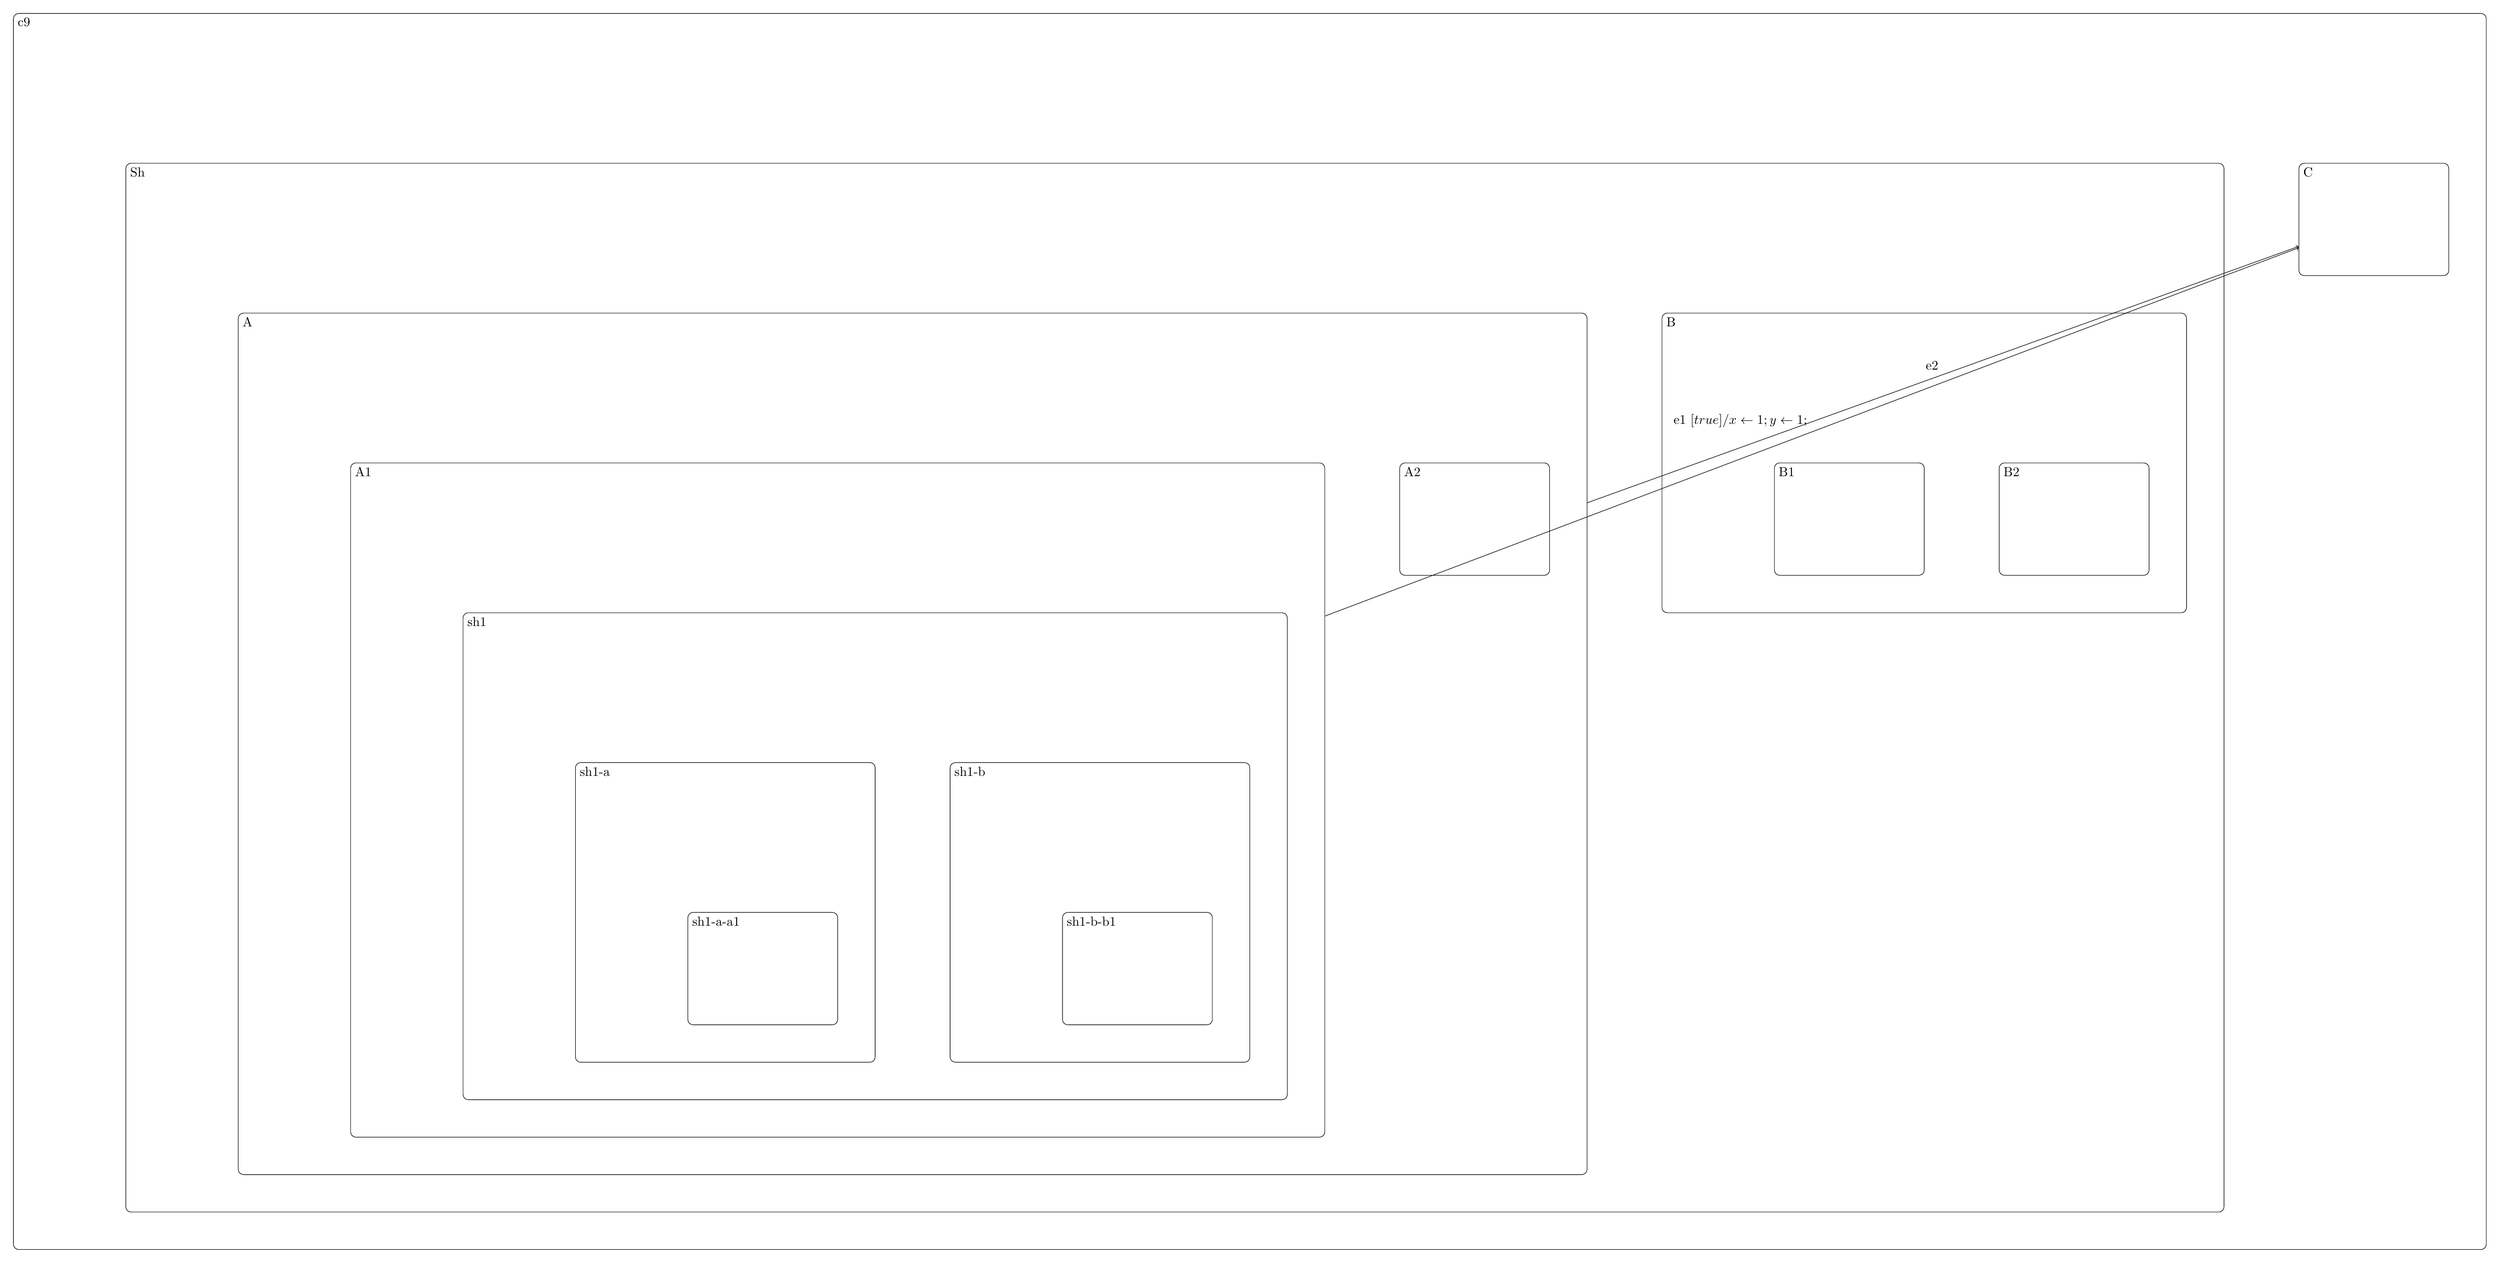
\begin{tikzpicture}[node distance=3cm, auto]
		\node[draw, rectangle, rounded corners, minimum width=66cm, minimum height=33cm, anchor=north west, label={[anchor=north west] north west:c9}] (c9) at (0, 0) {};
		\node[draw, rectangle, rounded corners, minimum width=56cm, minimum height=28cm, anchor=north west, label={[anchor=north west] north west:Sh}] (c9_Sh) at (3, -4) {};
		\node[draw, rectangle, rounded corners, minimum width=36cm, minimum height=23cm, anchor=north west, label={[anchor=north west] north west:A}] (c9_Sh_A) at (6, -8) {};
		\node[draw, rectangle, rounded corners, minimum width=26cm, minimum height=18cm, anchor=north west, label={[anchor=north west] north west:A1}] (c9_Sh_A_A1) at (9, -12) {};
		\node[draw, rectangle, rounded corners, minimum width=22cm, minimum height=13cm, anchor=north west, label={[anchor=north west] north west:sh1}] (c9_Sh_A_A1_sh1) at (12, -16) {};
		\node[draw, rectangle, rounded corners, minimum width=8cm, minimum height=8cm, anchor=north west, label={[anchor=north west] north west:sh1-a}] (c9_Sh_A_A1_sh1_sh1_a) at (15, -20) {};
		\node[draw, rectangle, rounded corners, minimum width=4cm, minimum height=3cm, anchor=north west, label={[anchor=north west] north west:sh1-a-a1}] (c9_Sh_A_A1_sh1_sh1_a_sh1_a_a1) at (18, -24) {};
		\node[draw, rectangle, rounded corners, minimum width=8cm, minimum height=8cm, anchor=north west, label={[anchor=north west] north west:sh1-b}] (c9_Sh_A_A1_sh1_sh1_b) at (25, -20) {};
		\node[draw, rectangle, rounded corners, minimum width=4cm, minimum height=3cm, anchor=north west, label={[anchor=north west] north west:sh1-b-b1}] (c9_Sh_A_A1_sh1_sh1_b_sh1_b_b1) at (28, -24) {};
		\node[draw, rectangle, rounded corners, minimum width=4cm, minimum height=3cm, anchor=north west, label={[anchor=north west] north west:A2}] (c9_Sh_A_A2) at (37, -12) {};
		\node[draw, rectangle, rounded corners, minimum width=14cm, minimum height=8cm, anchor=north west, label={[anchor=north west] north west:B}] (c9_Sh_B) at (44, -8) {};
		\node[draw, rectangle, rounded corners, minimum width=4cm, minimum height=3cm, anchor=north west, label={[anchor=north west] north west:B1}] (c9_Sh_B_B1) at (47, -12) {};
		\node[draw, rectangle, rounded corners, minimum width=4cm, minimum height=3cm, anchor=north west, label={[anchor=north west] north west:B2}] (c9_Sh_B_B2) at (53, -12) {};
		\node[draw, rectangle, rounded corners, minimum width=4cm, minimum height=3cm, anchor=north west, label={[anchor=north west] north west:C}] (c9_C) at (61, -4) {};
		\draw[->] (c9_Sh_A_A1) edge node  {e1 {$[true]  / x \leftarrow 1; y \leftarrow 1;$}} (c9_C);
		\draw[->] (c9_Sh_A) edge node  {e2} (c9_C);
	\end{tikzpicture}
\end{document}
